\documentclass[12pt]{article}
\usepackage[utf8]{inputenc}
\usepackage[spanish, es-tabla]{babel}
\usepackage{amsmath}
\usepackage{amsthm}
\usepackage{amsfonts}
\usepackage{amssymb}
\usepackage{tikz}
\usepackage{algpseudocode}
\usepackage{multicol}
\usepackage{multirow}
\usepackage{hhline}
\usepackage{natbib}
\usepackage{siunitx}
\usepackage{graphicx}
\usepackage{booktabs}
\usepackage{subfig}
\usepackage{tcolorbox}
\usepackage[shortlabels]{enumitem}
\usepackage{url}
\usepackage{circuitikz}
\usepackage{mathrsfs}

\usetikzlibrary{calc,arrows}

\setlength{\textwidth}{18cm}
\setlength{\oddsidemargin}{-1cm}
\setlength{\headsep}{-1cm}
\setlength{\voffset}{0cm}
\setlength{\topmargin}{0cm}
\setlength{\headheight}{0cm}
\textheight23cm

\graphicspath{{media/}}
\spanishdecimal{.}

\begin{document}
\colorbox{white!10!}{
    \begin{minipage}[t]{0.150 \textwidth}
       \begin{flushright}
        \includegraphics[width=0.6in]{ipn-national-polytechnic-institute-logo}
       \end{flushright}
    \end{minipage}
    \begin{minipage}[H]{0.62 \textwidth}
        \begin{center}
            {\large \textsc{Instituto Politécnico Nacional
            \\Escuela superior de ingeniería mecánica y eléctrica\\
            Unidad Zacatenco}}
            \vspace{0.25cm}
            \\
            { \large \textbf{Titulo del reporte}}
            \\
            \vspace{0.25cm}
            
            \textbf{Materia y otros datos}
            \vspace{0.10cm}
            \\
            Coloque aqui su nombre
            \\
            \today 
        \end{center}
        \vspace{0.05cm}
    \end{minipage}
    \begin{minipage}[t]{0.150 \textwidth}
        \begin{flushleft}
            \includegraphics[width=1in]{esime-logo.png}
        \end{flushleft}
    \end{minipage}
}

\paragraph{} Ejemplo de una ecuacion (distribucion de MB)
\begin{equation}
    n(u) = \frac{2N\pi}{\left(\pi kT\right)^{\frac{3}{2}}} \sqrt{u} \; e^{-\frac{u}{kT}}
\end{equation}
Como el primer término este compuesto de valores constantes, se establece C 
\begin{equation*}
    C =  \frac{2N\pi}{\left(\pi kT\right)^{\frac{3}{2}}}
\end{equation*}
Entonces se tendra una funcion 
\begin{equation*}
    u(x) = C\sqrt{x}\; e^{-x} \; ; \; x = \frac{u}{kT}
\end{equation*}
Esta función se grafica dando a C valor $C = 1$, para $x = [0,10]$, 
lo que da como resultado la grafica de la figura \ref{fig1}. 
\begin{figure}[h]
    \centering
    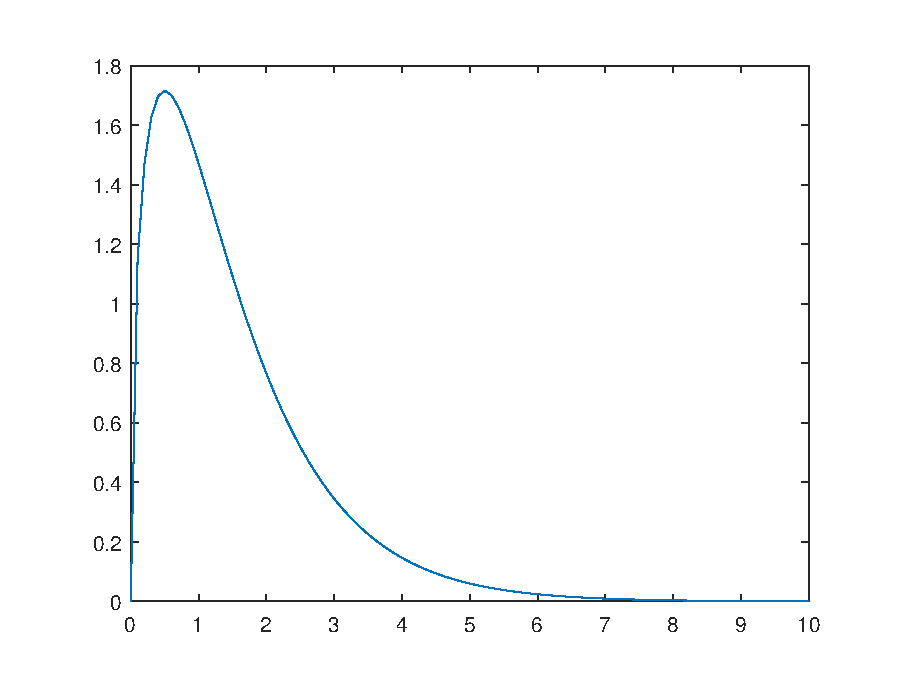
\includegraphics[scale = 0.5]{grafica.eps}
    \caption{Grafica de $u(x)$}
    \label{fig1}
\end{figure} 
\newpage
Ejemplo de tabla referenciada. Tabla \ref{tab1}
    \begin{table}[h]
        \centering
        \begin{tabular}{@{}ll@{}}
        \toprule
        $x$    & $u(x)$ \\ \midrule
        0      & 0      \\
        1.1111 & 0.347  \\
        2.2222 & 0.1615 \\
        3.3333 & 0.0561 \\
        4.4444 & 0.0248 \\
        5.5555 & 0.0091 \\
        6.6666 & 0.0033 \\
        7.7777 & 0.0012 \\
        8.8888 & 0.0004 \\
        10     & 0      \\ \bottomrule
        \end{tabular}
        \caption{Datos para $x = [0,10]$}
        \label{tab1}
        \end{table}
        
\end{document}